\section{Phân tích trường hợp}\label{sec:cases}
Bảng~\ref{tab:xai-cases} xét mười caption trong lượt khảo sát XAI ở seed 0, gồm năm trường hợp ảnh đứng đầu khớp ID ảnh chuẩn và năm trường hợp khác ID. Đây là cách phân nhóm theo đáp án của benchmark, không phải phán quyết ảnh khác ID sai về ngữ nghĩa. Hạng trong bảng là hạng của ảnh chuẩn theo QA-Graph trước can thiệp; các nhãn ở cột cuối là cạnh \texttt{contains} nối nhãn với ảnh đứng đầu được chọn khi cho phép tối đa ba cạnh. Vì vậy bảng mô tả quyết định đang được giải thích, không diễn giải các nhãn ấy như một quan hệ hành động đã được kiểm chứng.

\begin{table*}[t]
\caption{Mười trường hợp của QA-Graph trên VG$\cap$COCO và PSG$\cap$COCO, seed 0. ``Khớp'' nghĩa là ảnh đứng đầu trùng ID ảnh chuẩn; hạng là của ảnh chuẩn trước can thiệp. Nhãn liệt kê các cạnh \texttt{contains} được chọn để giải thích ảnh đứng đầu, tối đa ba cạnh.}\label{tab:xai-cases}
\centering\footnotesize
\begin{adjustbox}{max width=\textwidth}
\begin{tabular}{llcL{7.3cm}L{4.0cm}}
\toprule
Bộ & Khớp ID & Hạng & Truy vấn & Nhãn nối tới ảnh đứng đầu\\\midrule
VG & Có & 1 & several people hold umbrellas in a rain storm & umbrella, rain, people\\
VG & Có & 1 & A black and white photo of a building with a clock on it & clock, building, window\\
VG & Có & 1 & Car buried in snow next to what might be a gas pump & car, snow, meter\\
PSG & Có & 1 & A horse walks between cars in a parking lot & horse, car, road\\
PSG & Có & 1 & A man walking down the street carrying a suitcase & suitcase, person, pavement\\\midrule
VG & Không & 11 & Two zebras and another animal grazing in the grass & zebra, antelope, grass\\
VG & Không & 20 & a giraffe in an enclosure at an animal park & giraffe, zebra, fence\\
PSG & Không & 13 & A person sits on top of a motorcycle with others & motorcycle, person, road\\
PSG & Không & 13 & A group of women playing video games together & remote, person, tv\\
PSG & Không & 20 & There are many people on this field flying kites & kite, person, grass\\\bottomrule
\end{tabular}
\end{adjustbox}
\end{table*}

Hình~\ref{fig:xai-cases-match} và Hình~\ref{fig:xai-cases-mismatch} minh họa cả mười trường hợp trong Bảng~\ref{tab:xai-cases}. Nhóm khớp ID có một ảnh cho mỗi truy vấn; nhóm khác ID đặt ảnh đứng đầu cạnh ảnh chuẩn để có thể đối chiếu trực quan. Các nhãn trong hình là những cạnh \texttt{contains} nối nhãn với ảnh đứng đầu, không biểu diễn quan hệ giữa các đối tượng.
\begin{figure*}[t]
\centering
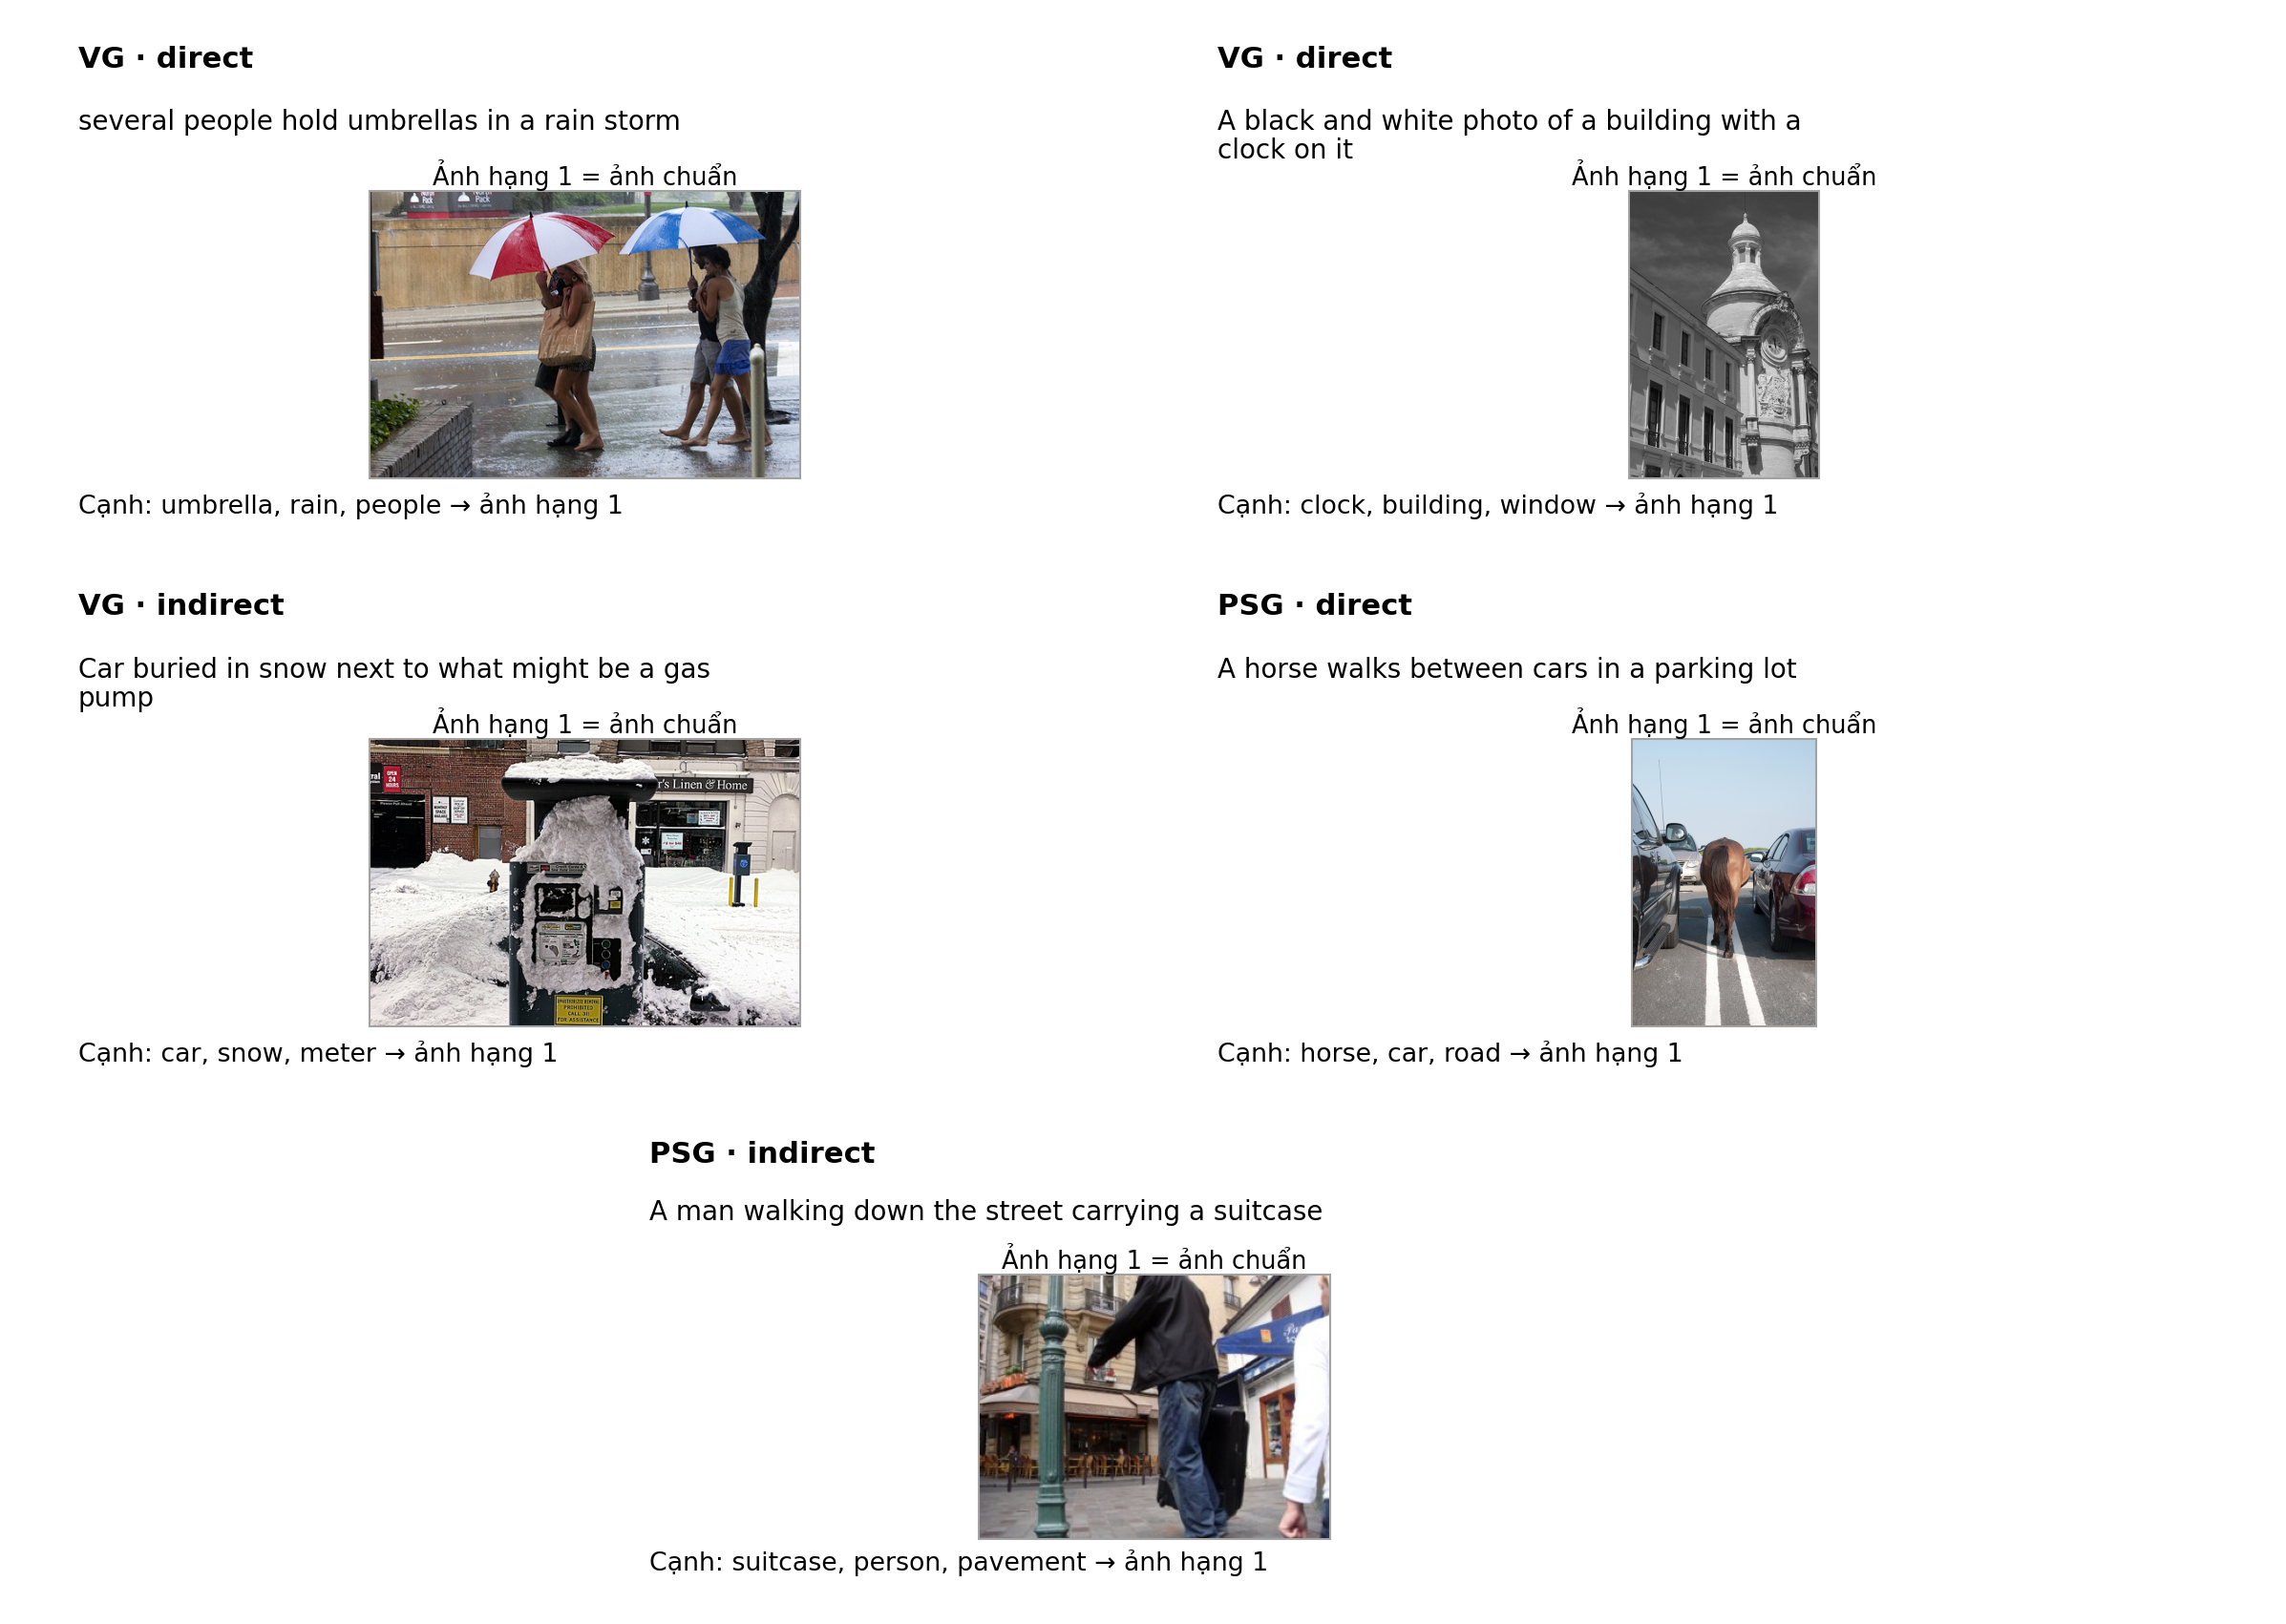
\includegraphics[width=\textwidth]{figs/xai_cases_match.png}
\caption{Năm trường hợp ảnh đứng đầu khớp ID ảnh chuẩn, gồm ba truy vấn VG$\cap$COCO và hai truy vấn PSG$\cap$COCO, seed 0. Dòng nhãn dưới mỗi ảnh liệt kê các cạnh \texttt{contains} được chọn để giải thích ảnh đứng đầu.}\label{fig:xai-cases-match}
\end{figure*}
\begin{figure*}[t]
\centering
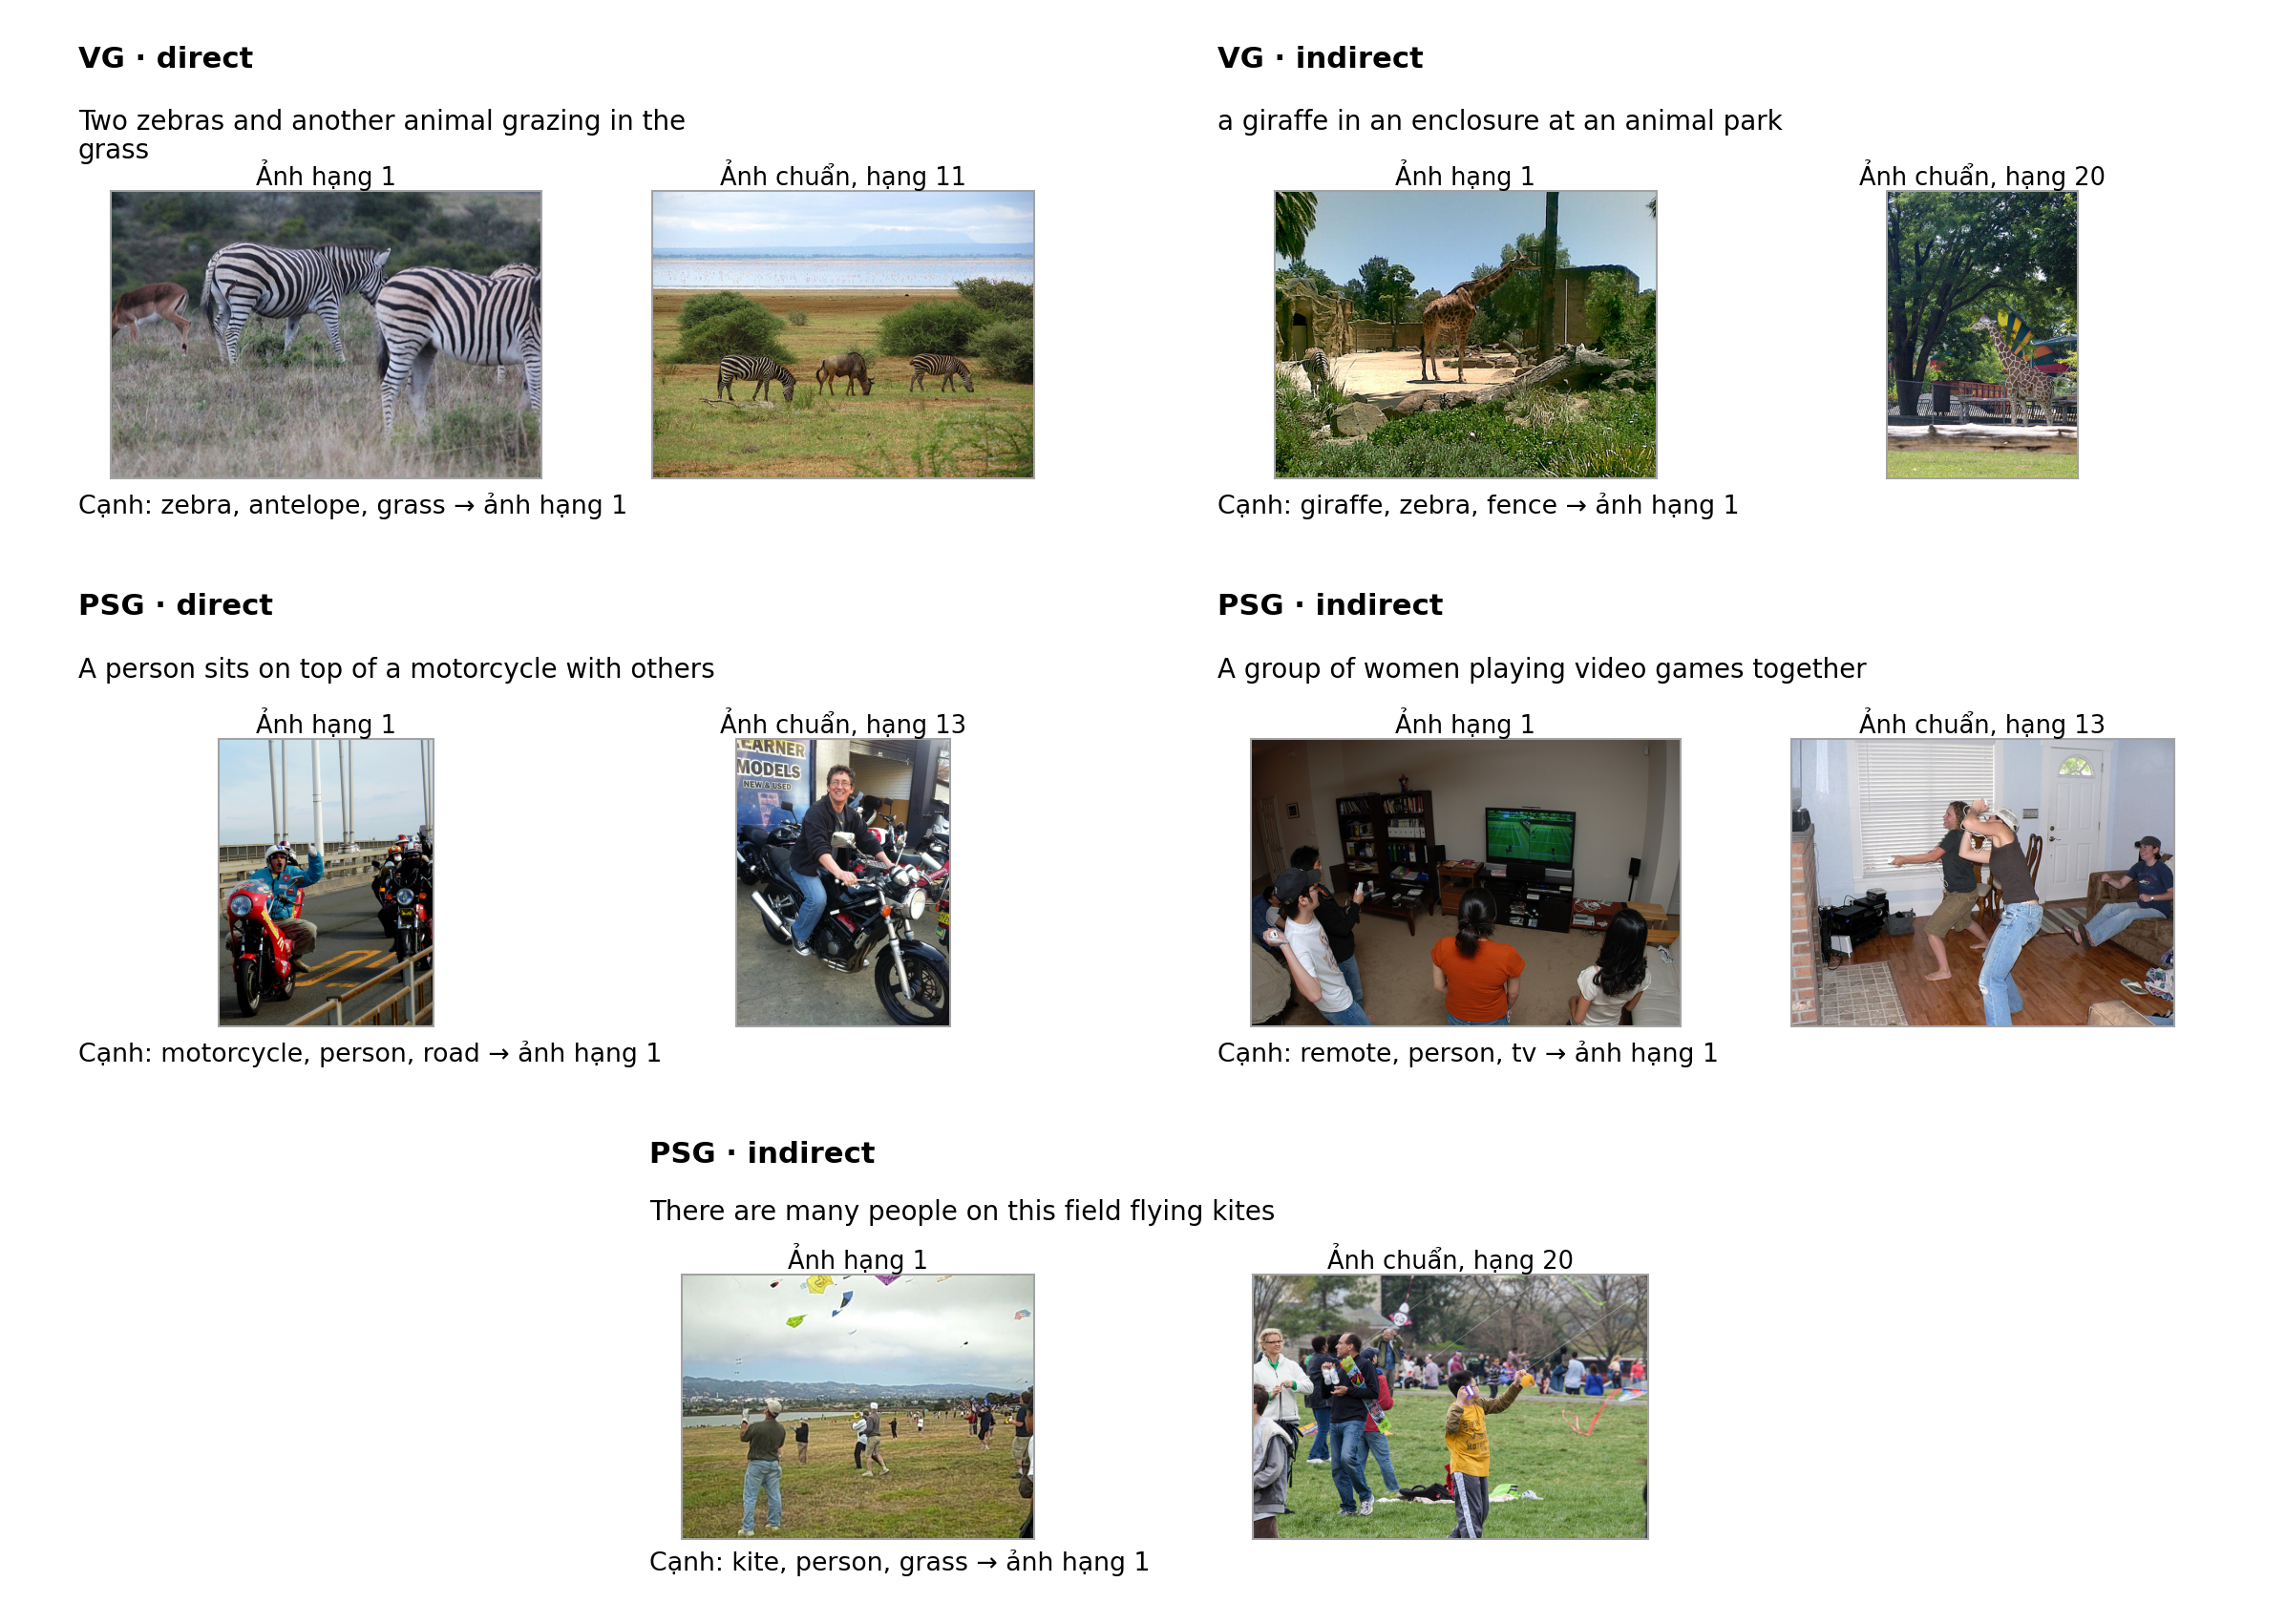
\includegraphics[width=\textwidth]{figs/xai_cases_mismatch.png}
\caption{Năm trường hợp ảnh đứng đầu khác ID ảnh chuẩn, gồm hai truy vấn VG$\cap$COCO và ba truy vấn PSG$\cap$COCO, seed 0. Hạng của ảnh chuẩn được ghi cạnh ảnh; dòng nhãn dưới mỗi cặp ảnh giải thích ảnh đứng đầu. Khác ID không tự chứng minh ảnh đứng đầu sai về ngữ nghĩa.}\label{fig:xai-cases-mismatch}
\end{figure*}

Ở năm trường hợp khớp ID, các nhãn được chọn bao phủ những đối tượng hoặc bối cảnh nổi bật của truy vấn: \emph{umbrella}, \emph{rain}, \emph{people} cho cảnh mưa; \emph{clock}, \emph{building}, \emph{window} cho tòa nhà; và \emph{car}, \emph{snow}, \emph{meter} cho cảnh xe trong tuyết. Hai truy vấn PSG cũng có các nhãn tương ứng là \emph{horse}, \emph{car}, \emph{road} và \emph{suitcase}, \emph{person}, \emph{pavement}. Xóa ba cạnh đã chọn ở trường hợp ô che mưa làm ảnh chuẩn từ hạng 1 xuống hạng 8; ở trường hợp người mang vali, ảnh chuẩn từ hạng 1 xuống hạng 4. Tác động lên thứ hạng cho thấy vai trò của nhãn đối tượng, còn thuộc tính đen trắng, vị trí ``giữa các xe'' và hành động ``mang vali'' chưa được các cạnh này kiểm chứng.

Ở năm trường hợp khác ID, ảnh đứng đầu vẫn có nhiều nhãn khớp bề mặt truy vấn. Truy vấn về ngựa vằn có \emph{zebra}, \emph{antelope}, \emph{grass}; truy vấn về hươu cao cổ có \emph{giraffe}, \emph{zebra}, \emph{fence}. Hai ảnh chuẩn tương ứng ở hạng 11 và 20. Trên PSG, các truy vấn về xe máy, trò chơi điện tử và thả diều lần lượt được giải thích bằng \emph{motorcycle}, \emph{person}, \emph{road}; \emph{remote}, \emph{person}, \emph{tv}; và \emph{kite}, \emph{person}, \emph{grass}, trong khi ảnh chuẩn ở hạng 13, 13 và 20. Các nhãn cho thấy nguồn điểm của ảnh được chọn, nhưng không xác nhận số lượng người, hành động hay quan hệ không gian mà câu truy vấn yêu cầu.

Một lượt rà ảnh khác, gồm mười truy vấn trực tiếp được chọn cân bằng theo ID, ghi nhận 5/10 ảnh đứng đầu trùng ảnh chuẩn. Cả năm ảnh khác ID trong mẫu đó cũng được xác nhận bằng mắt là phù hợp với truy vấn; tổng cộng 10/10 ảnh được xem là phù hợp trong đúng mẫu đã chọn. Kết quả này cho thấy phép đo khớp ID có thể đánh giá thiếu sự phù hợp ngữ nghĩa, nhưng mẫu nhỏ và phân tầng trước nên không dùng để ước lượng độ chính xác ngữ nghĩa trên toàn bộ 34 truy vấn trực tiếp. Hai tập mười trường hợp phục vụ hai phân tích khác nhau và không được cộng gộp.
